\documentclass[11pt,aspectratio=169]{beamer}

\usepackage{slides}
\usepackage{soul}
\usepackage{pdfpc}
\usepackage{ebproof}
\usepackage{bigdelim}
\usepackage{booktabs}
\usepackage{listings}
\usepackage{tcolorbox}
\usepackage{tabularx}
\usepackage{tikz}
\usepackage{xspace}
\usepackage[T1]{fontenc}
\usepackage[utf8]{inputenc}
\usepackage[symbol]{footmisc}
\usepackage[noend]{algpseudocode}
\usepackage[
    backend    = biber,
    style      = alphabetic,
    giveninits = true,
    maxnames   = 16,
    minnames   = 16,
]{biblatex}

\addbibresource{./references.bib}

\usetikzlibrary{
    positioning,
    shapes.symbols,
    shadows,
    arrows,
    calc
}

\newcommand{\senc}{\text{senc}}
\newcommand{\msg}{\text{msg}}
\newcommand{\nonce}{\text{nonce}}
\newcommand{\KDF}{\text{KDF}}
\newcommand{\key}{\text{key}}

\newcommand{\Tamarin}[1]{\textsc{Tamarin}\xspace}

%% Print: [#1] -[#2]-> [#3]
\newcommand{\MSR}[3]{#1 -\hspace{-4pt}[\hspace{5pt} #2 \hspace{4pt}]\hspace{-4.6pt}\rightarrow #3}
%% Print: -[#1]->
\newcommand{\ActionFact}[1]{-\hspace{-4pt}[\hspace{5pt} #1 \hspace{4pt}]\hspace{-4.6pt}\rightarrow}
%% Print: ~
\newcommand{\tildelow}{\raisebox{0.5ex}{\texttildelow}}
%% Print: ^
\newcommand{\pow}{\textasciicircum{}}
%% Highlight text in overlay
\newcommand{\althl}[2][2]{\alt<#1>{\hl{#2}}{#2}}

%% Sticky notes to represent facts
\definecolor{StickyNoteYellow}{RGB}{241,239,161}
\definecolor{StickyNoteRed}{RGB}{255,167,169}
\definecolor{StickyNoteGreen}{RGB}{148,199,146}
\definecolor{StickyNoteBlue}{RGB}{167,229,241}
\NewDocumentCommand{\StickyNote}{O{StickyNoteYellow}O{1cm}m}{%
    \begin{tikzpicture}
        \node[
            drop shadow={
                shadow xshift = 2pt,
                shadow yshift = -4pt,
            },
            xslant = -0.1,
            yslant = 0.1,
            draw   = black,
            fill   = #1,
            text   = black,
        ] {\parbox[t][#2][c]{#2}{\centering#3}};
    \end{tikzpicture}
}

%% Colors for terms and facts
\definecolor{TermBlue}{HTML}{1C377D}
\definecolor{FactPurple}{HTML}{7C3655}

\newcommand{\term}[1]{\textcolor{TermBlue}{#1}}
\newcommand{\Term}[1]{\textcolor{TermBlue}{#1}}
\newcommand{\Fact}[1]{\textcolor{FactPurple}{#1}}

%% Other colors
\definecolor{AdversaryRed}{HTML}{DA3B26}

%% Listings
\lstset{escapeinside={(*@}{@*)}}
\lstset{numberstyle=\tiny}

\definecolor{TamarinBlue}{RGB}{42,0,255}
\definecolor{TamarinGreen}{RGB}{48,110,32}
\definecolor{TamarinPurple}{RGB}{175,36,67}

\lstdefinestyle{tamarin}{
    basicstyle    = \linespread{0.75}\footnotesize\ttfamily,
    extendedchars = true,
    tabsize       = 2,
    columns       = fixed,
    numbers       = none,
    breaklines    = true,
    literate      = {~}{{\raisebox{0.5ex}{\texttildelow}}}{1},
    morekeywords  = {theory, builtins, restriction, equations, functions, rule,
                     let, in, lemma, All, Ex, not, predicates, begin, end},
    keywordstyle  = \color{TamarinPurple},
    morecomment   = [l]{//},
    morecomment   = [s]{/*}{*/},
    commentstyle  = \color{TamarinGreen},
    xleftmargin   = 0mm,
    upquote       = true,
    morestring    = *[b]",
    showstringspaces = false
}

\lstdefinestyle{tactic}{
    basicstyle    = \linespread{0.75}\footnotesize\ttfamily,
    extendedchars = true,
    tabsize       = 2,
    columns       = fixed,
    numbers       = none,
    breaklines    = true,
    literate      = {~}{{\raisebox{0.5ex}{\texttildelow}}}{1},
    alsoletter    = :,
    morekeywords  = {tactic:, presort:, prio:, deprio:},
    keywordstyle  = \color{TamarinPurple},
    morecomment   = [l]{//},
    morecomment   = [s]{/*}{*/},
    commentstyle  = \color{TamarinGreen},
    xleftmargin   = 0mm,
    upquote       = true,
    morestring    = *[b]",
}

\lstdefinestyle{oracle}{
    basicstyle    = \linespread{0.75}\footnotesize\ttfamily,
    extendedchars = true,
    tabsize       = 2,
    columns       = fixed,
    numbers       = none,
    breaklines    = true,
    literate      = {~}{{\raisebox{0.5ex}{\texttildelow}}}{1},
    morecomment   = [l]{\#},
    morekeywords  = {import, for, in, if, elif},
    keywordstyle  = \color{TamarinPurple},
    commentstyle  = \color{TamarinGreen},
    xleftmargin   = 0mm,
    upquote       = true,
}

\definecolor{ProVerifGreen}{RGB}{48,110,32}
\definecolor{ProVerifBlue}{RGB}{64,112,161}

\lstdefinestyle{proverif}{
    basicstyle    = \linespread{0.75}\footnotesize\ttfamily,
    extendedchars = true,
    tabsize       = 2,
    columns       = fixed,
    numbers       = none,
    breaklines    = true,
    literate      = {~}{{\raisebox{0.5ex}{\texttildelow}}}{1},
    morecomment   = [s]{(*}{*)},
    commentstyle  = \color{ProVerifGreen},
    keywordstyle  = \color{ProVerifBlue},
    morekeywords  = {in, if, event, new, let, out},
    xleftmargin   = 0mm,
}

\definecolor{proofTreeBlue}{HTML}{2639B0}
\definecolor{proofTreeRed}{HTML}{921C12}

\lstdefinestyle{prooftree}{
    basicstyle    = \linespread{0.8}\footnotesize\fontfamily{pcr}\selectfont,
    extendedchars = true,
    tabsize       = 2,
    columns       = fixed,
    numbers       = left,
    breaklines    = true,
    literate      = {~}{{\raisebox{0.5ex}{\texttildelow}}}{1},
    keywords      = [1]{lemma, case, next, qed, by, end, Diff-Lemmas},
    keywordstyle  = [1]\color{black}\bfseries,
    keywords      = [2]{simplify, solve, sorry, contradiction, induction,
                        autoprove, rule-equivalence},
    keywordstyle  = [2]\color{proofTreeBlue}\bfseries,
    keywords      = [3]{@, \|, <, \^},
    keywordstyle  = [3]\color{proofTreeRed},
    alsoletter    = @\|<\^-,
    moredelim     = **[is][{\color{proofTreeBlue}}]{<<}{>>},
    xleftmargin   = 0mm,
    upquote       = true,
    morestring    = *[b]",
}

%% Color boxes
\definecolor{ColorBoxBlue}{HTML}{1C377D}
\tcbset{
    colback      = white,
    colframe     = black,
    fonttitle    = \bfseries,
    coltitle     = white,
    colbacktitle = ColorBoxBlue,
    boxrule      = 1pt
}

%% Vertical separator for frames
\newcommand<>{\vsep}{
    \begin{tikzpicture}[remember picture,overlay]%
        \draw[ultra thick]
            ($(current page.north west)+(8cm,0.5cm)$) to
            ($(current page.south west)+(8cm,-0.5cm)$)
        ;
    \end{tikzpicture}%
}

%% Horizontal separator for frames
\newcommand<>{\hsep}{
    \begin{tikzpicture}[remember picture,overlay]%
        \draw[ultra thick]
            ($(current page.north west)+(-0.5cm,-4.5cm)$) to
            ($(current page.north east)+(0.5cm,-4.5cm)$)
        ;
    \end{tikzpicture}%
}


\title{Formal Analysis of Real-World Security Protocols}
\subtitle{Lecture 0: Organization and Motivation}
\date{\today}
\author{Aleksi Peltonen}
\institute{CISPA Helmholtz Center for Information Security}

\begin{document}
\maketitle

% ---------------------------------------------------------------------------- %
% Content
% ---------------------------------------------------------------------------- %

\begin{frame}[fragile]{What is a protocol?}
    \begin{itemize}
        \item<1-> A \textbf{protocol} is a set of rules that determine how two 
                  or more parties can achieve a common goal by exchanging 
                  messages
        \item<2-> Protocols that use cryptography to achieve security-related 
                  goals are called \textbf{security} or \textbf{cryptographic} 
                  protocols
    \end{itemize}
    \begin{figure}
        \includegraphics<1>[width=.5\textwidth]{figures/lecture_0/protocol_1}%
        \includegraphics<2>[width=.5\textwidth]{figures/lecture_0/protocol_2}
    \end{figure}
\end{frame}

\begin{frame}[t,fragile]{Why should we care about protocol security?}
    \begin{itemize}
        \item New things are constantly connected to the Internet \\- security 
              \alt<2>{\textbf{\textcolor{AdversaryRed}{threats}}}
              {\textbf{protocols}} are everywhere
    \end{itemize}
    \vfill
    \begin{figure}
        \includegraphics<1>[width=.7\textwidth]
            {figures/lecture_0/connected_devices}%
        \includegraphics<2>[width=.7\textwidth]
            {figures/lecture_0/articles}%
    \end{figure}
\end{frame}

% ---------------------------------------------------------------------------- %

\section{How do we know a protocol is secure?}

% ---------------------------------------------------------------------------- %

\begin{frame}[fragile,b]{Before 1970}
    \begin{itemize}
        \item \textbf{No proofs}
        \item Trial and error -- we're not quite sure what a clever attacker 
              could do
        \item Security: break - patch - repeat
    \end{itemize}
    \vfill
    \begin{figure}
        \includegraphics<0>[width=.7\textwidth]
            {figures/lecture_0/protocol_development_1}%
        \includegraphics<1>[width=.7\textwidth]
            {figures/lecture_0/protocol_development_2}
    \end{figure}
\end{frame}

\begin{frame}[fragile,b]{1970-1980}
    \begin{itemize}
        \item \textbf{Let's prove security} (Goldwasser, Micali, Yao)
        \item Attacker is any polynomial-time Turing machine
        \item Reduce security problem to generically solving a hard problem\\ 
              (e.g., discrete logarithm, factoring)
    \end{itemize}
    \vfill
    \begin{figure}
        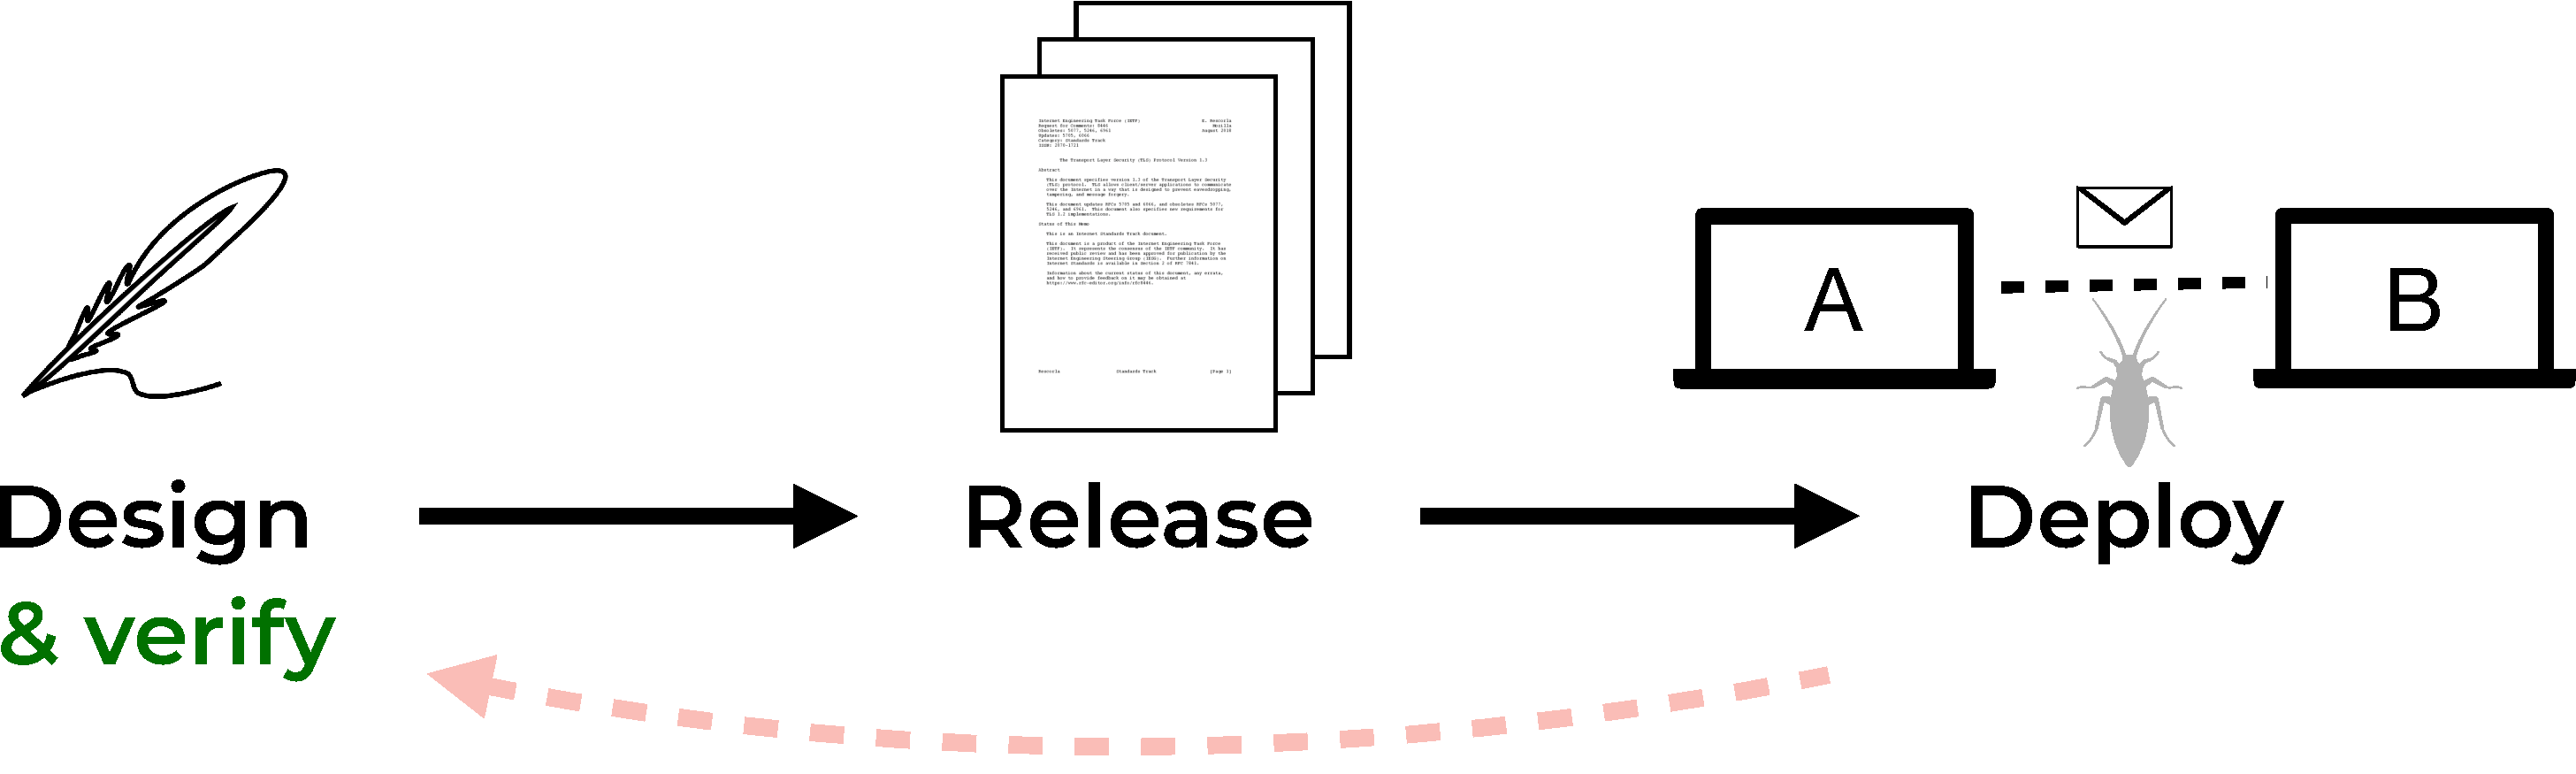
\includegraphics[width=.7\textwidth]
            {figures/lecture_0/protocol_development_3}
    \end{figure}
\end{frame}

\begin{frame}[fragile]{1980-1990}
    \begin{itemize}
        \item \textbf{Computational proofs}
        \begin{itemize}
            \item Proofs scale from primitives (``a signature scheme'') to 
                  small protocols (``a simple key exchange protocol'')
            \item Typically pen-and-paper proofs, very error prone
            \item \textit{Not the focus of this lecture}
        \end{itemize}
        \item \textbf{Symbolic proofs}
        \begin{itemize}
            \item 1983: symbolic attacker model (Dolev-Yao)
            \item Reason about abstract terms instead of bitstrings
            \item ``Perfect cryptography'' assumption: Attacker can only 
                  decrypt an encrypted message if they know the key
            \item Example property: Show that attacker can (not) learn a secret 
                  term
        \end{itemize}
    \end{itemize}
\end{frame}

\begin{frame}[fragile]{1990-2000}
    \begin{itemize}
        \item \textbf{Model checkers become more widespread}
        \begin{itemize}
            \item Analyze small finite cases
            \item Found many flaws on basic designs
                \begin{itemize}
                    \item 1995: MitM attack on the NSPK protocol discovered 
                          with automated verification
                \end{itemize}
        \end{itemize}
        \item \textbf{Proliferation of tools \& methods}
        \begin{itemize}
            \item CSP/FDR, Prolog, NRL Protocol Analyzer, $\dots$
            \item BAN Logic and variants
            \item Isabelle (Paulson)
        \end{itemize}
    \end{itemize}
\end{frame}

\begin{frame}[fragile]{2000-2010}
    \begin{columns}
        \begin{column}{0.5\textwidth}
            \begin{itemize}
                \item \textbf{Bounded analysis matures}
                \begin{itemize}
                    \item AVISPA/Avantssar (OFMC, SAT-MC, CL-Atse)
                    \item Hit scaling barrier: State space explosion
                \end{itemize}
                \item \textbf{Unbounded analysis?}
                \begin{itemize}
                    \item Undecidable.. Yet workable in practice?
                    \item ProVerif, Maude-NPA, Scyther, CPSA, Athena
                \end{itemize}
            \end{itemize}
        \end{column}
        \begin{column}{0.5\textwidth}
            \begin{figure}
                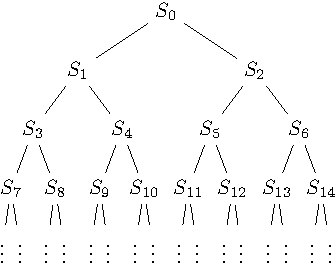
\includegraphics[width=.8\textwidth]
                    {./figures/lecture_0/state_space_explosion}
            \end{figure}
        \end{column}
    \end{columns}
\end{frame}

\begin{frame}[fragile]{2010-}
    \begin{columns}
        \begin{column}{0.7\textwidth}
            \begin{itemize}
                \item Tool situation stabilizes
                \begin{itemize}
                    \item ProVerif
                    \item \textbf{Tamarin prover}
                \end{itemize}
                \item Increased expressiveness
                \begin{itemize}
                    \item Equational theories
                    \item Loops / stateful protocols
                \end{itemize}
                \item \textbf{Real-world analysis}
                \begin{itemize}
                    \item Scaling to real-world protocols
                    \item Stronger threat models
                    \item Visibility to security engineers and standards bodies
                \end{itemize}
            \end{itemize}
        \end{column}
        \begin{column}{0.3\textwidth}
            
\includegraphics[width=0.5\textwidth]
                {./figures/lecture_0/proverif_logo}\\[.5cm]
            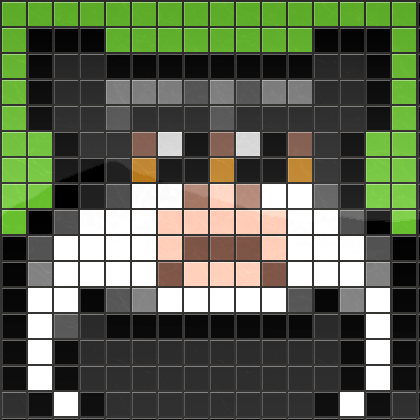
\includegraphics[width=0.5\textwidth]
                {./figures/lecture_0/tamarin_logo_pixel}
        \end{column}
    \end{columns}
\end{frame}

% ---------------------------------------------------------------------------- %

\section{Course Overview}

% ---------------------------------------------------------------------------- %

\begin{frame}[fragile]{This lecture}
    \begin{tikzpicture}[remember picture, overlay]
        \node[below left] at (current page.north east) {
            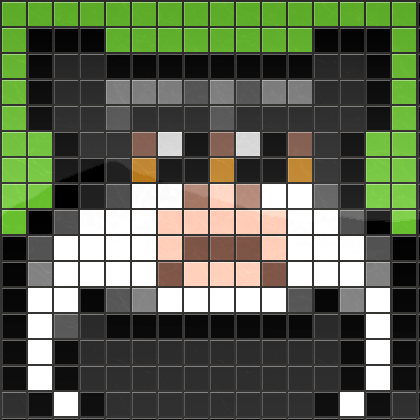
\includegraphics[width=0.1\textwidth]
                {./figures/lecture_0/tamarin_logo_pixel}
        };
    \end{tikzpicture}
    \begin{itemize}
        \item What is formal analysis of security protocols?
        \item Learn about one state-of-the-art tool: the \textbf{Tamarin prover}
        \begin{itemize}
            \item Learn how Tamarin works
            \item Learn how to use Tamarin
            \item Analyze protocols!
        \end{itemize}
        \item Understand the \textbf{guarantees} and \textbf{limitations} of 
              such analyses
        \item How have they been applied to \textbf{real-world protocols}?
        \item What \textbf{research} still needs to be done to make protocols 
              secure?
    \end{itemize}
\end{frame}

\begin{frame}[fragile]{Lecture plan}
    \begin{table}[]\scriptsize
        \vspace*{-.2cm}
        \begin{tabular}{rl}
            \textbf{Lecture} & \textbf{Content} \\
            \toprule
            0 & Organization and Motivation \\ \midrule
            1 & Terms and Equational Theories \\
            2 & Protocols in the Symbolic Model \\
            3 & Attacker Model and Trace Properties \\
            4 & Verification Theory (Part 1) \\
            5 & Verification Theory (Part 2) \\ \midrule
            6 & Using Tamarin in Practice \\
            7 & Advanced Security Properties and Threat Models \\
            8 & Advanced Features (Part 1) \\
            9 & Advanced Features (Part 2) \\ \midrule
            10 & Security Protocol Standards \\
            11 & Relation to Cryptography, Scaling, and the Future \\
            \bottomrule
        \end{tabular}
    \end{table}
\end{frame}

\begin{frame}[fragile]{Course book}
    \begin{itemize}
        \item David Basin, Cas Cremers, Jannik Dreier, and Ralf Sasse.
              \textbf{Modeling and Analyzing Security Protocols with Tamarin:
                      A Comprehensive Guide}.
        \begin{itemize}
            \item Available online:
                  \url{https://tamarin-prover.com/book/index.html}
            \item Each lecture will have a list of references to the relevant
                  sections (based on v0.9.5)
        \end{itemize}
    \item Other references will be included as additional reading when necessary
    \end{itemize}
\end{frame}

% ---------------------------------------------------------------------------- %

\section{Analysis of Real-World Protocols}

% ---------------------------------------------------------------------------- %

\begin{frame}[fragile]{The Tamarin prover}
    \begin{columns}
        \begin{column}{0.6\textwidth}
            \begin{itemize}
                \item Symbolic analysis of security protocols
                \item First released in 2012, still under active development
                \item Simple protocols: Fully automatic
                \item Complex protocols: Interactive mode
                \item Considers an \textbf{unbounded number of sessions}, 
                      supports advanced features like stateful protocols and 
                      loops
                \item Open source on GitHub: \url{https://tamarin-prover.com/}
            \end{itemize}
        \end{column}
        \begin{column}{0.4\textwidth}
            \begin{figure}
                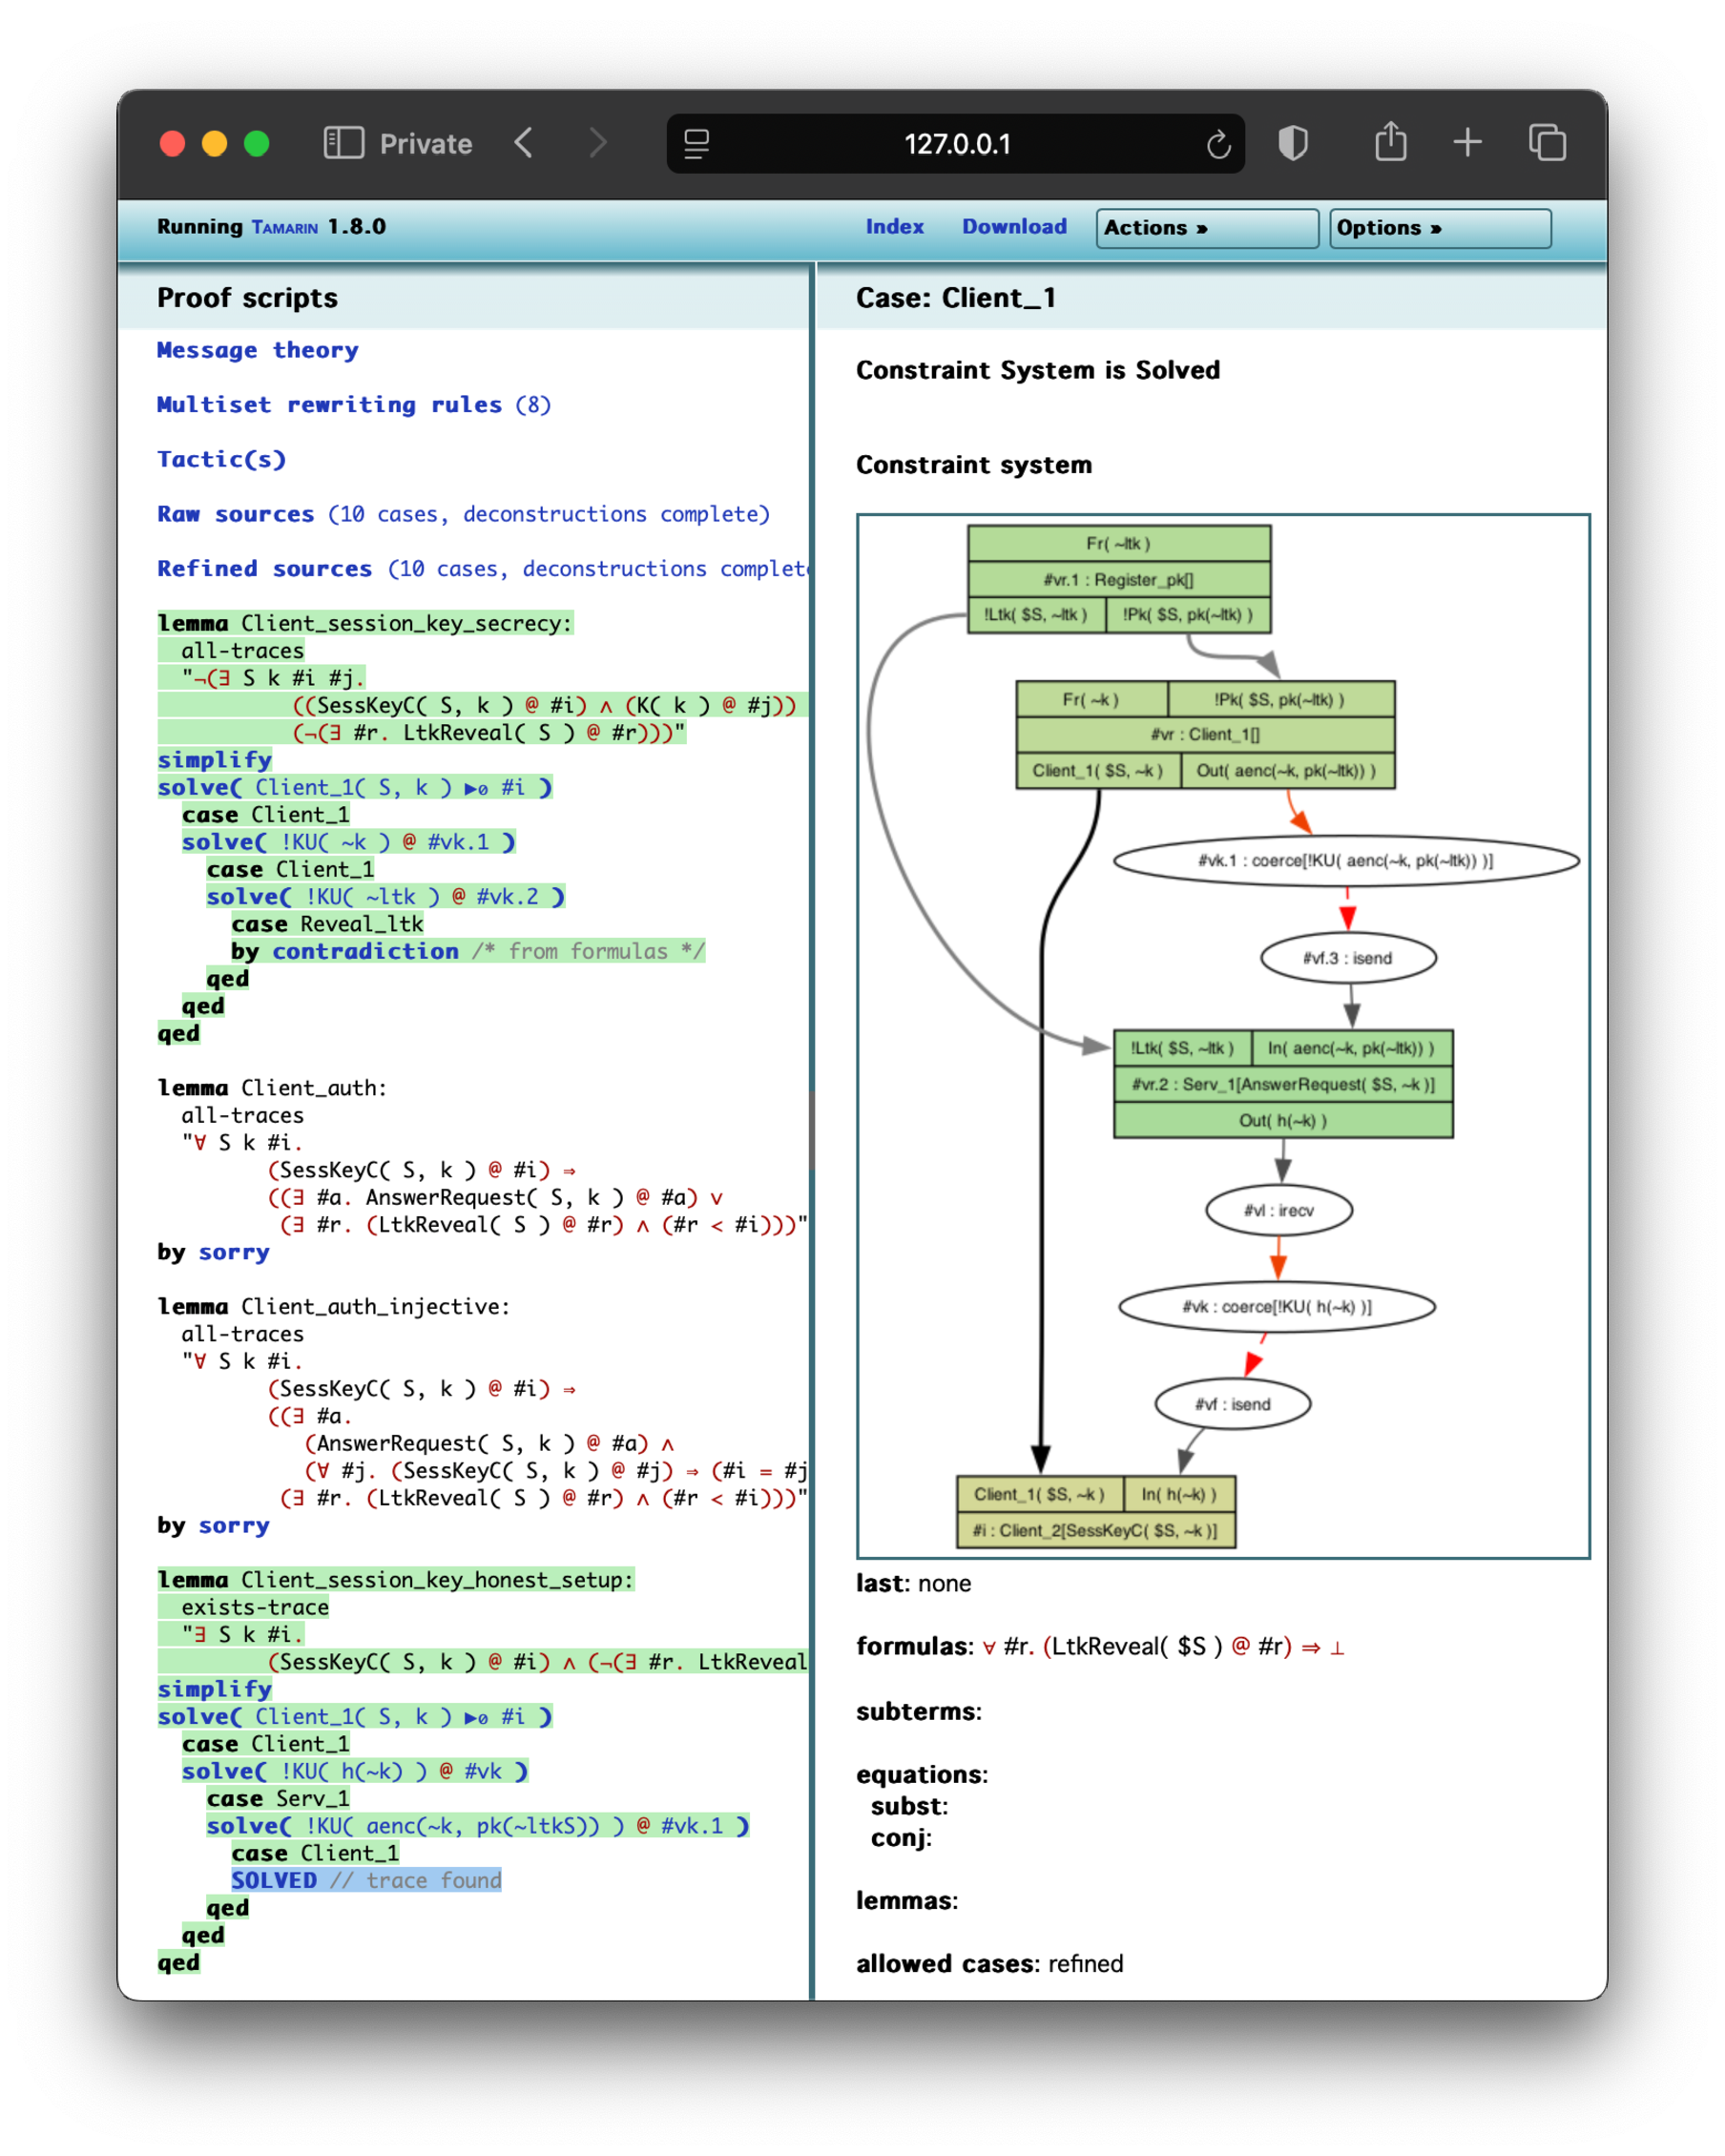
\includegraphics[width=.95\textwidth]
                    {./figures/lecture_0/tamarin_gui}
            \end{figure}
        \end{column}
    \end{columns}
    \begin{tikzpicture}[remember picture, overlay]
        \node[below left] at (current page.north east) {
            \frame{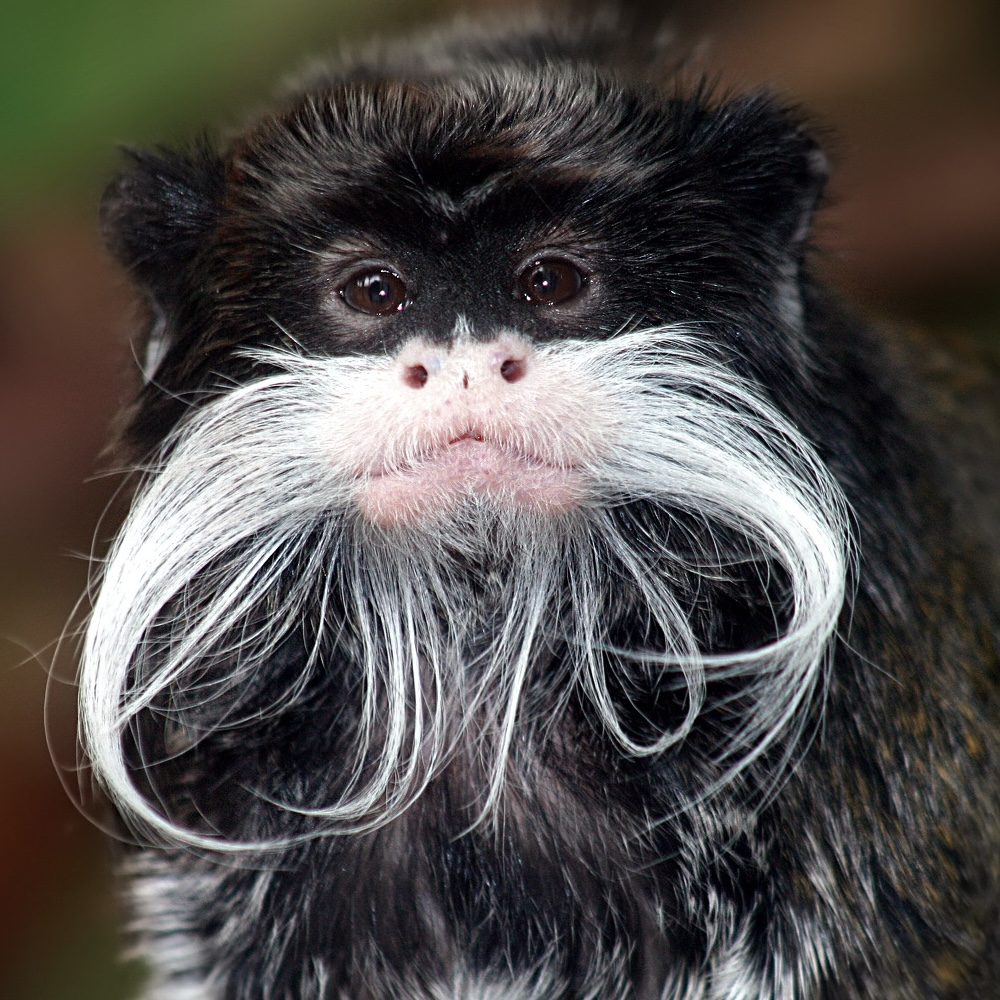
\includegraphics[width=0.08\textwidth]
                {./figures/lecture_0/tamarin_photo_small}}
            \frame{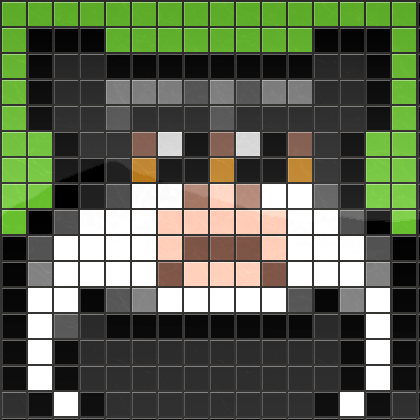
\includegraphics[width=0.08\textwidth]
                {./figures/lecture_0/tamarin_logo_pixel}}
        };
    \end{tikzpicture}
\end{frame}

\begin{frame}[fragile]{The Tamarin prover}
    \begin{tikzpicture}[remember picture, overlay]
        \node[left, yshift=.5cm] (img) at (current page.center) {
            \includegraphics<1>[width=0.4\textwidth]
                {./figures/lecture_0/tamarin_photo_hatless}%
            \includegraphics<2>[width=0.4\textwidth]
                {./figures/lecture_0/tamarin_photo_hat}
        };
        \draw[
            line width=1mm,
            triangle 45-,
            color=orange,
        ] (img.east) +(0,-1.8) -- +(2,-1.8) node[right] {Constraint solver};
        \only<2>{
            \draw[
                line width=1mm,
                triangle 45-,
                color=orange,
            ] (img.east) +(0,-.3) -- +(2,-.3) node[right] {Theorem prover};
        }
    \end{tikzpicture}
\end{frame}

\begin{frame}[fragile]{Application domain examples}
    \begin{columns}
        \begin{column}{0.36\textwidth}
            \textbf{Key Exchange}
            \begin{itemize}
                \item \colorbox{white}{Naxos}
                \item \colorbox{white}{Signed DH}
                \item \colorbox{white}{Station-to-Station}
                \item \colorbox{white}{IKEv2}
                \item \colorbox{white}{Wireguard}
                \item \colorbox{white}{PQ-Wireguard}
                \item \colorbox{white}{Noise protocol family}
            \end{itemize}
        \end{column}
        \begin{column}{0.36\textwidth}
            \textbf{Large Case Studies}
            \begin{itemize}
                \item \only<1>{\colorbox{white}{TLS 1.3}}
                      \only<2>{\colorbox{blue!20}{TLS 1.3}}
                \item \colorbox{white}{IEEE 802.11 WPA2}
                \item \only<1>{\colorbox{white}{5G-AKA}}
                      \only<2>{\colorbox{blue!20}{5G-AKA}}
                \item \colorbox{white}{5G handover}
                \item \colorbox{white}{SPDM 1.2}
                \item \colorbox{white}{Apple iMessage PQ3}
            \end{itemize}
            \textbf{Payment}
            \begin{itemize}
                \item \only<1>{\colorbox{white}{EMV}}
                      \only<2>{\colorbox{blue!20}{EMV}}
            \end{itemize}
        \end{column}
        \begin{column}{0.3\textwidth}
            \textbf{Authentication}
            \begin{itemize}
                \item \colorbox{white}{WS-Security}
                \item \colorbox{white}{ACME}
            \end{itemize}
            \textbf{E-voting}
            \begin{itemize}
                \item \colorbox{white}{Alethea}
                \item \colorbox{white}{Belenios}
                \item \colorbox{white}{Selene}
            \end{itemize}
            \textbf{PKI}
            \begin{itemize}
                \item \colorbox{white}{ARPKI}
            \end{itemize}
        \end{column}
    \end{columns}
\end{frame}

\begin{frame}[fragile]{Example 1 - TLS 1.3}
    \begin{itemize}
        \item \textbf{What is it?}
        \begin{itemize}
            \item \textbf{T}ransport \textbf{L}ayer \textbf{S}ecurity, version 
                  \textbf{1.3}
            \item Likely the world's most used security protocol
        \end{itemize}
        \item \textbf{Tamarin analysis}
        \begin{itemize}
            \item Explicit support for the IETF during the development of
                  TLS 1.3
            \item Several person months of work: much of it in just 
                  understanding the standard
        \end{itemize}
        \item \textbf{Results}
        \begin{itemize}
            \item Tamarin finds complete break for the main proposal for
                  Rev 10+'s ``delayed authentication''
            \item Minimal attack involves 3 modes \& 18 messages
            \item Motivated change to other mechanism
            \item Proven core properties for final version
        \end{itemize}
    \end{itemize}
\end{frame}

\begin{frame}[fragile]{Example 2 - 5G-AKA}
    \begin{itemize}
        \item \textbf{What is it?}
        \begin{itemize}
            \item \textbf{5G} \textbf{A}uthentication and \textbf{K}ey\\
                  \textbf{A}greement
            \item The core key exchange of 5G
        \end{itemize}
        \item \textbf{Tamarin analysis}
        \begin{itemize}
            \item Analysis of the near-final standard (>1 000 pages)
            \item Standard notably harder to parse than TLS 1.3's RFC, yet 
                  semi-stable
        \end{itemize}
        \item \textbf{Results}
        \begin{itemize}
            \item Tamarin finds that privacy is not guaranteed (linkable)
                  -- needs redesign
            \item Tamarin proves other properties under some assumptions
            \item (Prediction: many current wontfix'es will cause trouble later)
        \end{itemize}
    \end{itemize}
    \begin{tikzpicture}[remember picture, overlay]
        \node[
            below left,
            xshift=-.25cm,
            yshift=-.25cm,
        ] at (current page.north east) {
            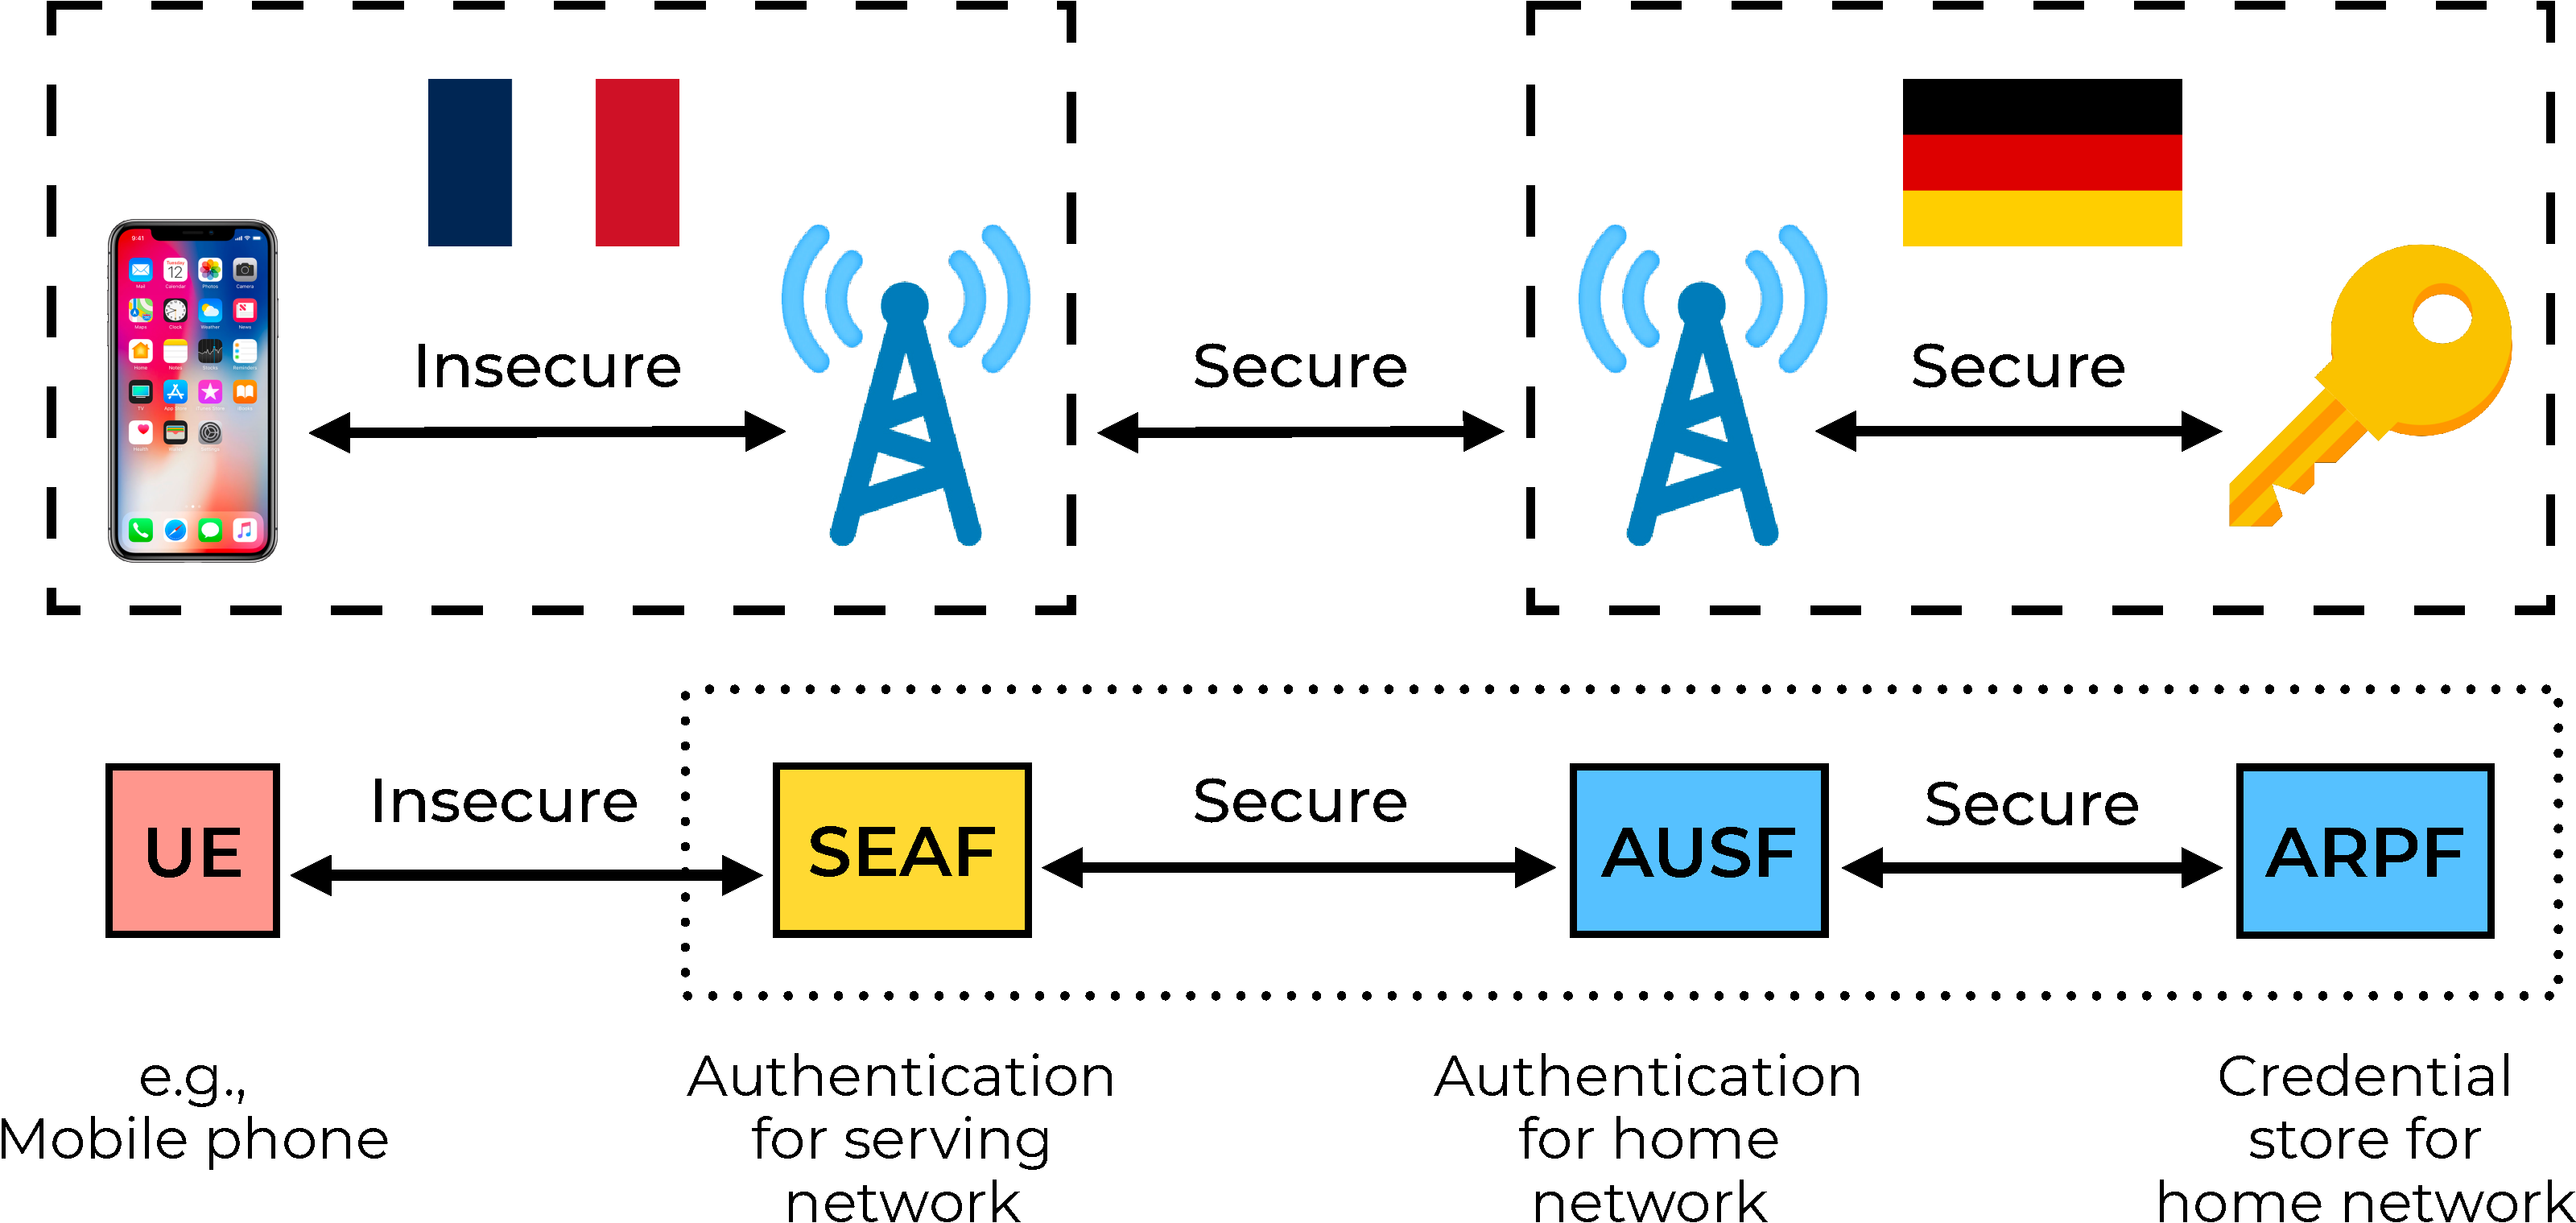
\includegraphics[width=0.5\textwidth]{./figures/lecture_0/5g-aka}
        };
    \end{tikzpicture}
\end{frame}

\begin{frame}[fragile]{Example 3 - EMV}
    \begin{itemize}
        \item \textbf{What is it?}
        \begin{itemize}
            \item \textbf{E}uropay, \textbf{M}astercard, and \textbf{V}isa
            \item Protocol between your bank, terminal, credit card
            \item Modern versions have many different modes: Contactless, PIN, 
                  etc.
        \end{itemize}
        \item \textbf{Tamarin analysis}
        \begin{itemize}
            \item Standard documentation complex
            \item Partial reverse engineering
        \end{itemize}
        \item \textbf{Results}
        \begin{itemize}
            \item Main attacks by researchers from ETH Z\"{u}rich
            \begin{itemize}
                \item PIN bypass: use man-in-the-middle to perform arbitrarily 
                      large transaction
                \item Card mixup attack allow bypassing PIN codes
            \end{itemize}
            \item Later refined attacks by researchers from Birmingham and 
                  Surrey
            \begin{itemize}
                \item Relay attacks and attacks on locked iPhones
            \end{itemize}
        \end{itemize}
    \end{itemize}
    \begin{tikzpicture}[remember picture, overlay]
        \node[
            below left,
            xshift=-.25cm,
            yshift=-.25cm,
        ] at (current page.north east) {
            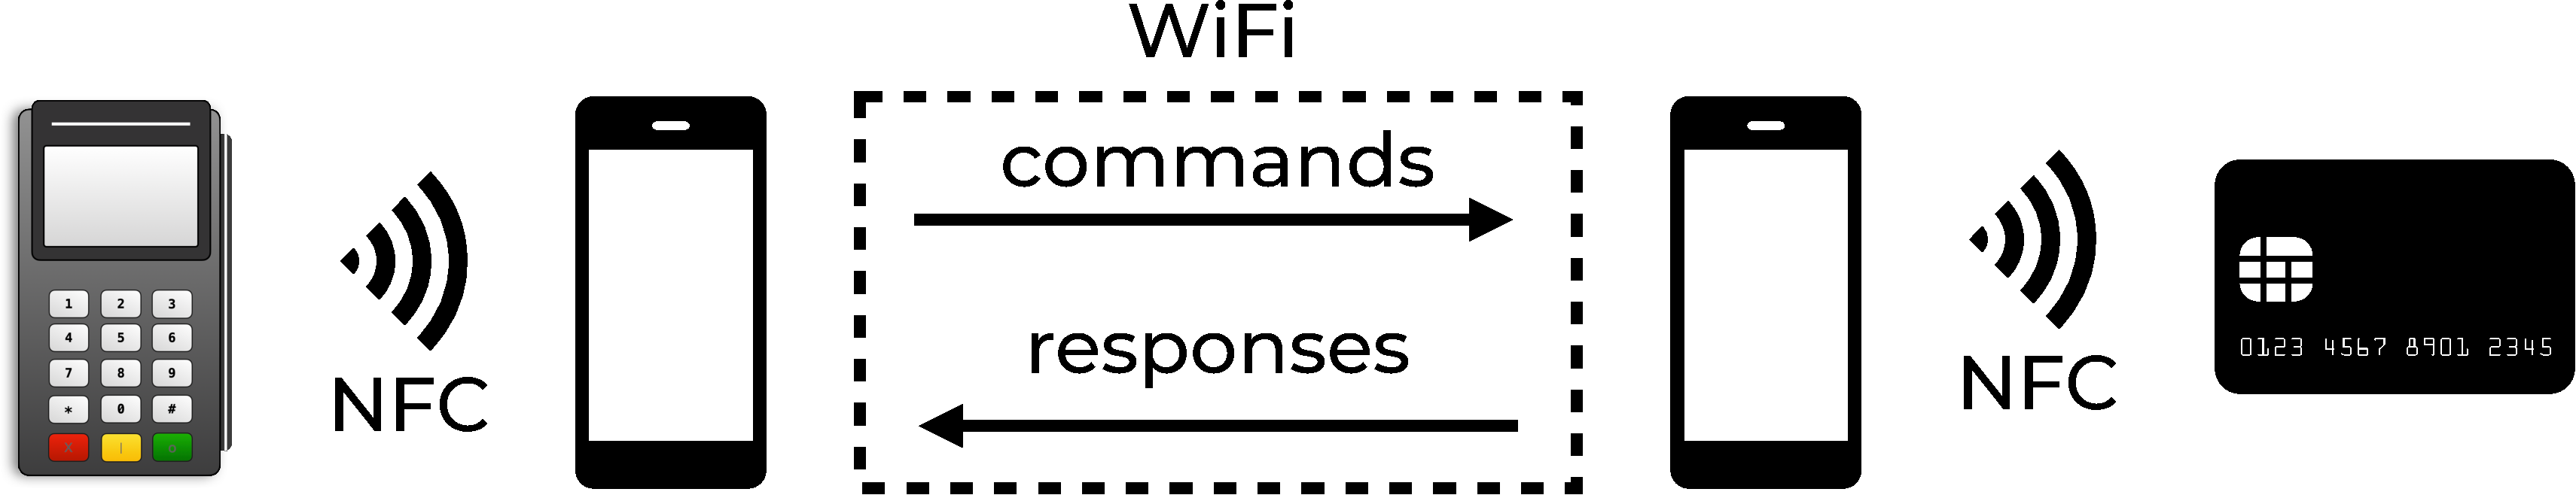
\includegraphics[width=0.5\textwidth]{./figures/lecture_0/emv}
        };
    \end{tikzpicture}
\end{frame}

% ---------------------------------------------------------------------------- %

\section{Back to Basics: Diffie-Hellman}

% ---------------------------------------------------------------------------- %

\begin{frame}[fragile]{Diffie-Hellman key exchange}
    \begin{columns}
        \begin{column}{0.5\hsize}
        One of the first proposals for secure protocols, for which we will see 
        several variants.
        \begin{itemize}
            \item ``g\pow{}x'' is shorthand for ``gx mod P'', where g is the 
                    generator of a prime order group of order P. It is
                    \textbf{efficient to compute g\pow{}x}
            \item If the group is sufficiently large, it is
                  \textbf{infeasible to compute x from g\pow{}x}
        \end{itemize}
        \end{column}
        \begin{column}{0.5\hsize}
            \begin{figure}
                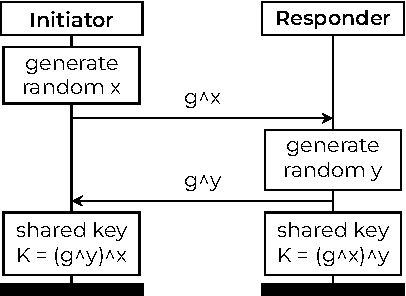
\includegraphics[width=\textwidth]{./figures/lecture_0/dh}
            \end{figure}
        \end{column}
    \end{columns}
\end{frame}

\begin{frame}[fragile]{Diffie-Hellman key exchange}
    \begin{columns}
        \begin{column}{0.5\hsize}
        What should this protocol achieve?
        \begin{itemize}
            \item If an adversary observes the network messages g\pow{}x and 
                  g\pow{}y, they cannot compute the shared key!
            \item What if the adversary can insert messages too?
        \end{itemize}
        \end{column}
        \begin{column}{0.5\hsize}
            \begin{figure}
                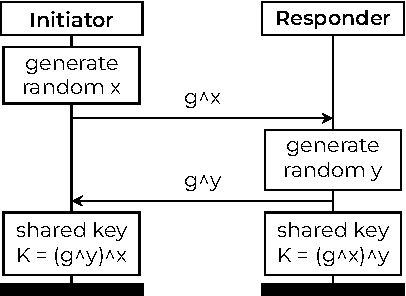
\includegraphics[width=\textwidth]{./figures/lecture_0/dh}
            \end{figure}
        \end{column}
    \end{columns}
\end{frame}

\begin{frame}[fragile]{Man-in-the-middle attack}
    \begin{figure}
        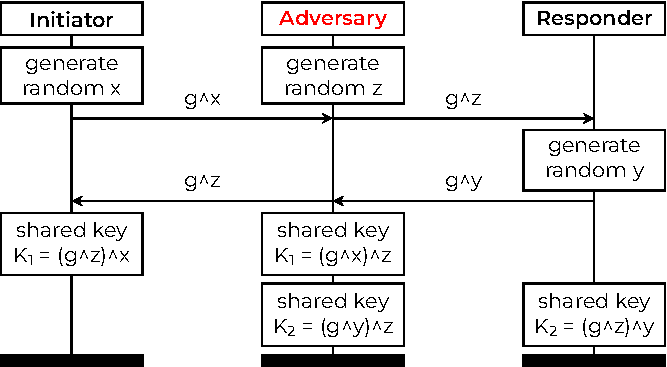
\includegraphics[width=.7\textwidth]{./figures/lecture_0/dh_mitm}
    \end{figure}
\end{frame}

\begin{frame}[fragile]{Execution model}
    \begin{figure}
        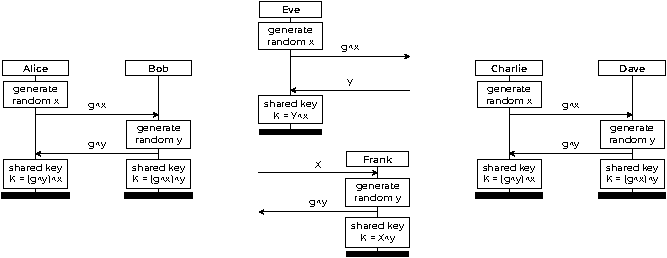
\includegraphics[width=\textwidth]{./figures/lecture_0/dh_exe}
    \end{figure}
\end{frame}

\begin{frame}[fragile]{Adversary view}
    \begin{figure}
        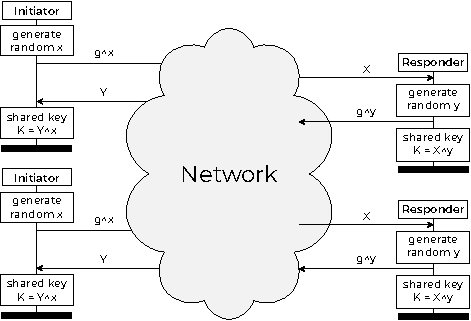
\includegraphics[width=.7\textwidth]{./figures/lecture_0/dh_adv}
    \end{figure}
\end{frame}

% ---------------------------------------------------------------------------- %

\section{Summary}

% ---------------------------------------------------------------------------- %

\begin{frame}[fragile]{Summary}
    \begin{columns}
        \begin{column}{0.65\textwidth}
            \begin{itemize}
                \item Today, we learned that..
                \begin{itemize}
                    \item ..protocol security can be analyzed computationally
                          or \textbf{symbolically}
                    \item ..we can automate the process using modern tools like 
                          \textbf{\Tamarin}
                \end{itemize}
                \item In the next lecture, we will learn more about modeling..
                \begin{itemize}
                    \item \textit{messages} as \textbf{terms}, and
                    \item \textit{cryptographic primitives} as
                          \textbf{equations}
                \end{itemize}
            \end{itemize}
        \end{column}
        \begin{column}{0.35\textwidth}
            \begin{figure}
                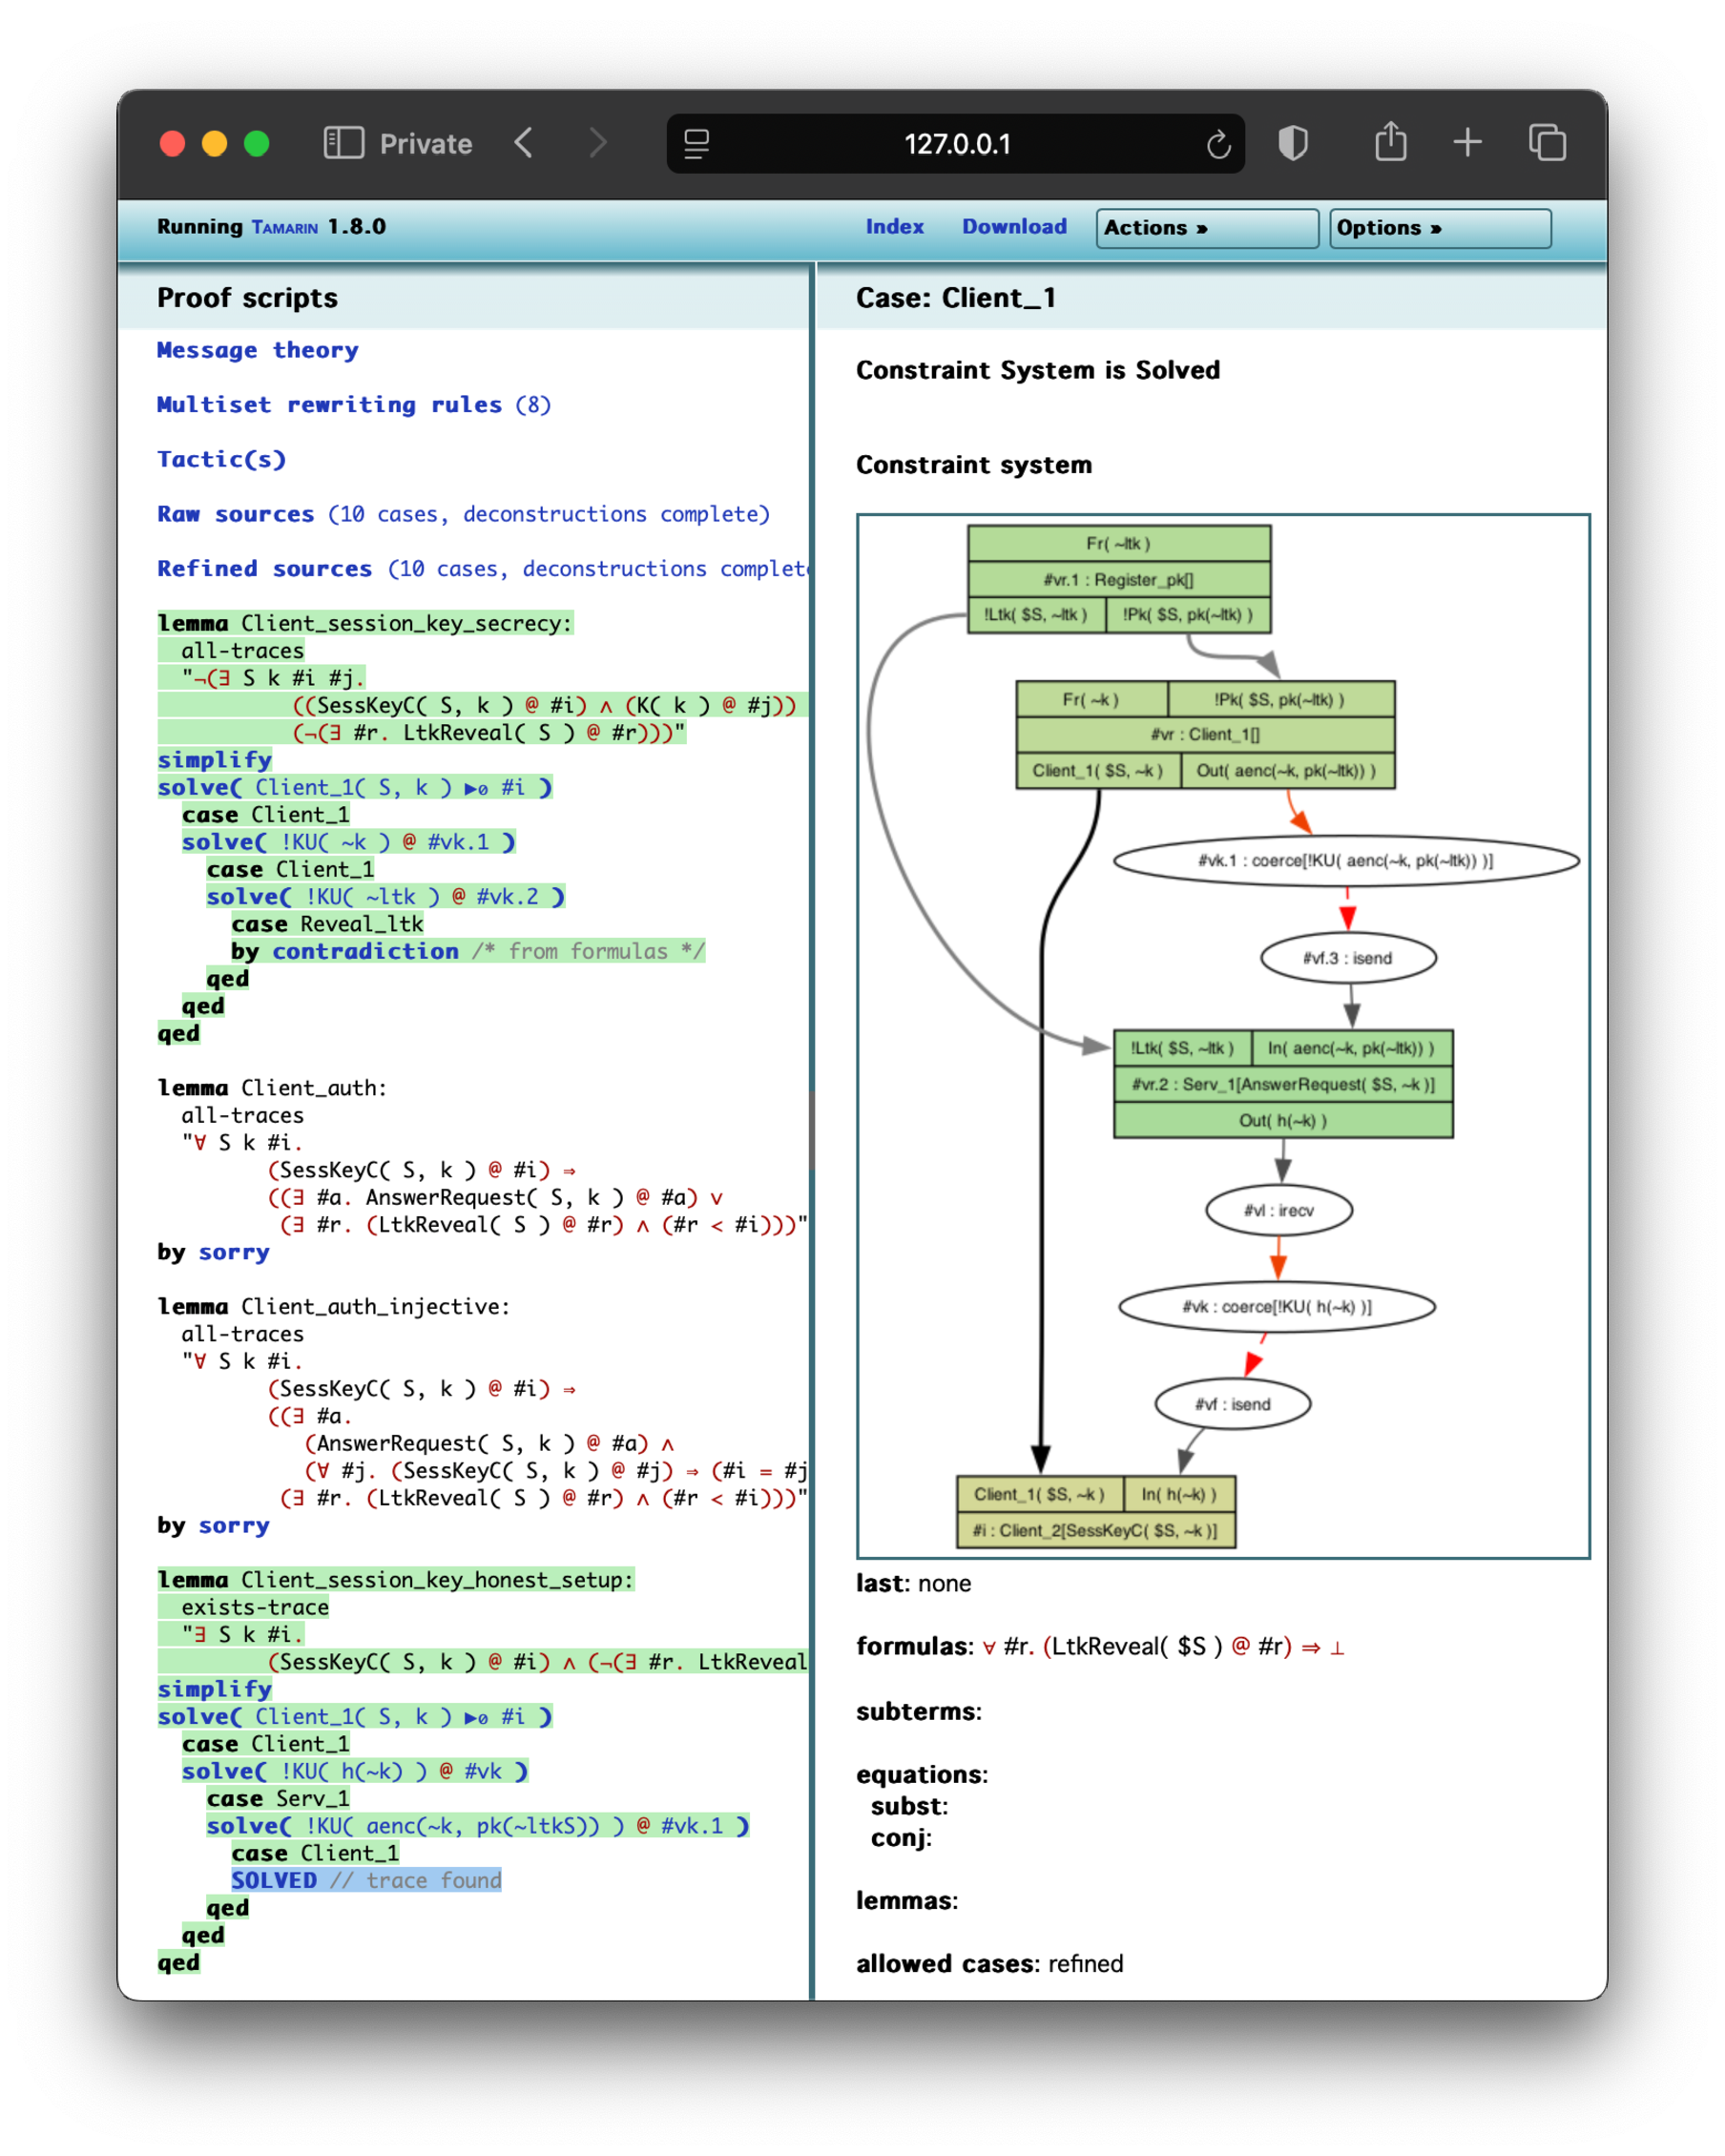
\includegraphics[width=.9\textwidth]
                    {./figures/lecture_0/tamarin_gui}
            \end{figure}
        \end{column}
    \end{columns}
    \begin{tikzpicture}[remember picture, overlay]
        \node[below left] at (current page.north east) {
            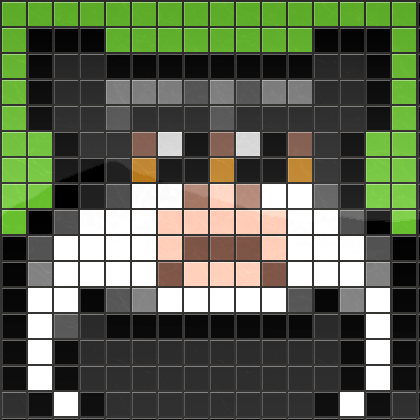
\includegraphics[width=0.08\textwidth]
                {./figures/lecture_0/tamarin_logo_pixel}
        };
    \end{tikzpicture}
\end{frame}

% ---------------------------------------------------------------------------- %
% Reading Material
% ---------------------------------------------------------------------------- %
\begin{frame}[fragile]{Reading material}
    \textbf{Recommended reading}:
        ~\cite[Ch. 1--2]{tamarin-book}
    \begin{refsection} 
        \nocite{tamarin-book}
        \printbibliography[heading=none]
    \end{refsection}
\end{frame}

\begin{frame}[allowframebreaks]{Case studies}
    \textbf{Case studies}:\\ \;
        TLS 1.3~\cite{cremers2016tls13,cremers2017tls13},\\ \;
        5G-AKA~\cite{basin20185gaka,cremers20195gaka},\\ \;
        EMV~\cite{basin2021emv,basin2021emvmixup,radu2022emv}
    \begin{refsection} 
        \nocite{cremers2016tls13,cremers2017tls13,basin20185gaka,
                cremers20195gaka,basin2021emv,basin2021emvmixup,radu2022emv}
        \printbibliography[heading=none]
    \end{refsection}
\end{frame}
% ---------------------------------------------------------------------------- %

\end{document}
